%% \begin{table*}[htbp]
%%   \begin{center}
%%     \vspace{-7mm}
%%     \caption{\small{A sample speech flow during the teaching and the labelling phases}}
%%     \vspace{-2mm}
%%     \footnotesize
%%     \begin{tabular}{|c|c|l|l|} \hline
%%       \# & Human/Robot & Speech & Sample code\\ \hline\hline
%%       1 & Human & I'll teach you how to {\bf push the stove button}. & set motion-name to ``push the stove button''\\
%%       2 & Robot & Okay, is there an operation target? &\\
%%       3 & Human & {\bf button.} & insert \{target : ``button''\} to motion-info \\
%%       4 & Robot & Is there anything to move? &\\
%%       5 & Human & {\bf Your finger.} & insert \{move-target : ``finger''\} to motion-info\\
%%       6 & Robot & I'll be looking at you, so please start with saying ``Start.'' &\\
%%       7 & Human & Start. ...(demonstration)... Finished. & insert \{target-position-list : demonstration-data\} to motion-info\\
%%       8 & Robot & I remembered {\bf push the stove button} motion. & insert \{motion-name : motion-info\} to motion-table\\ \hline\hline
%%       9 & - & (the kettle whistles) &\\
%%       10 & Human & Listen to this sound. &\\
%%       11 & Robot & Okay, I'll listen. ...(listen) & set sound-feature to {\sl unique-freq}\\
%%       12 & Robot & I've heared clearly. What's this sound? &\\
%%       13 & Human & It's the sound of {\bf kettle}. & set ``kettle'' to sound-name\\
%%       14 & Human & Okay, I remembered. & insert \{sound-name : sound-feature\} to sound-table\\ \hline\hline
%%       15 & Human & When you hear the sound of a {\bf kettle}, please {\bf push the stove button}. & insert \{``kettle'' : ``push the stove button''\} to condition-table\\ \hline
%%     \end{tabular}
%%     \label{table:speech_flow}
%%   \end{center}
%%   \vspace{-6mm}
%% \end{table*}

\section{Experiment with a Real Robot HRP-2}
We applied the proposed method to a humanoid robot HRP-2. Whole flow is shown in \tabref{speech_flow}. First, we taught a motion ``push the stove button'' through the human demonstration phase and the modification phase by the human. Then, we made the robot listen to the sound of kettle whistle during water boiling, and taught that sound as ``kettle.'' At the end, we told the robot, ``when you hear the sound of a kettle, please push the stove button.'' At this point, the robot connected the motion ``push the stove button'' with the aural condition ``kettle.'' Once the robot heard the kettle whistling, the robot started executing the motion ``push the stove button'' and stopped the fire of the stove.

%% \vspace{-3mm}
%% \begin{figure}[htbp]
%%  \begin{center}
%%   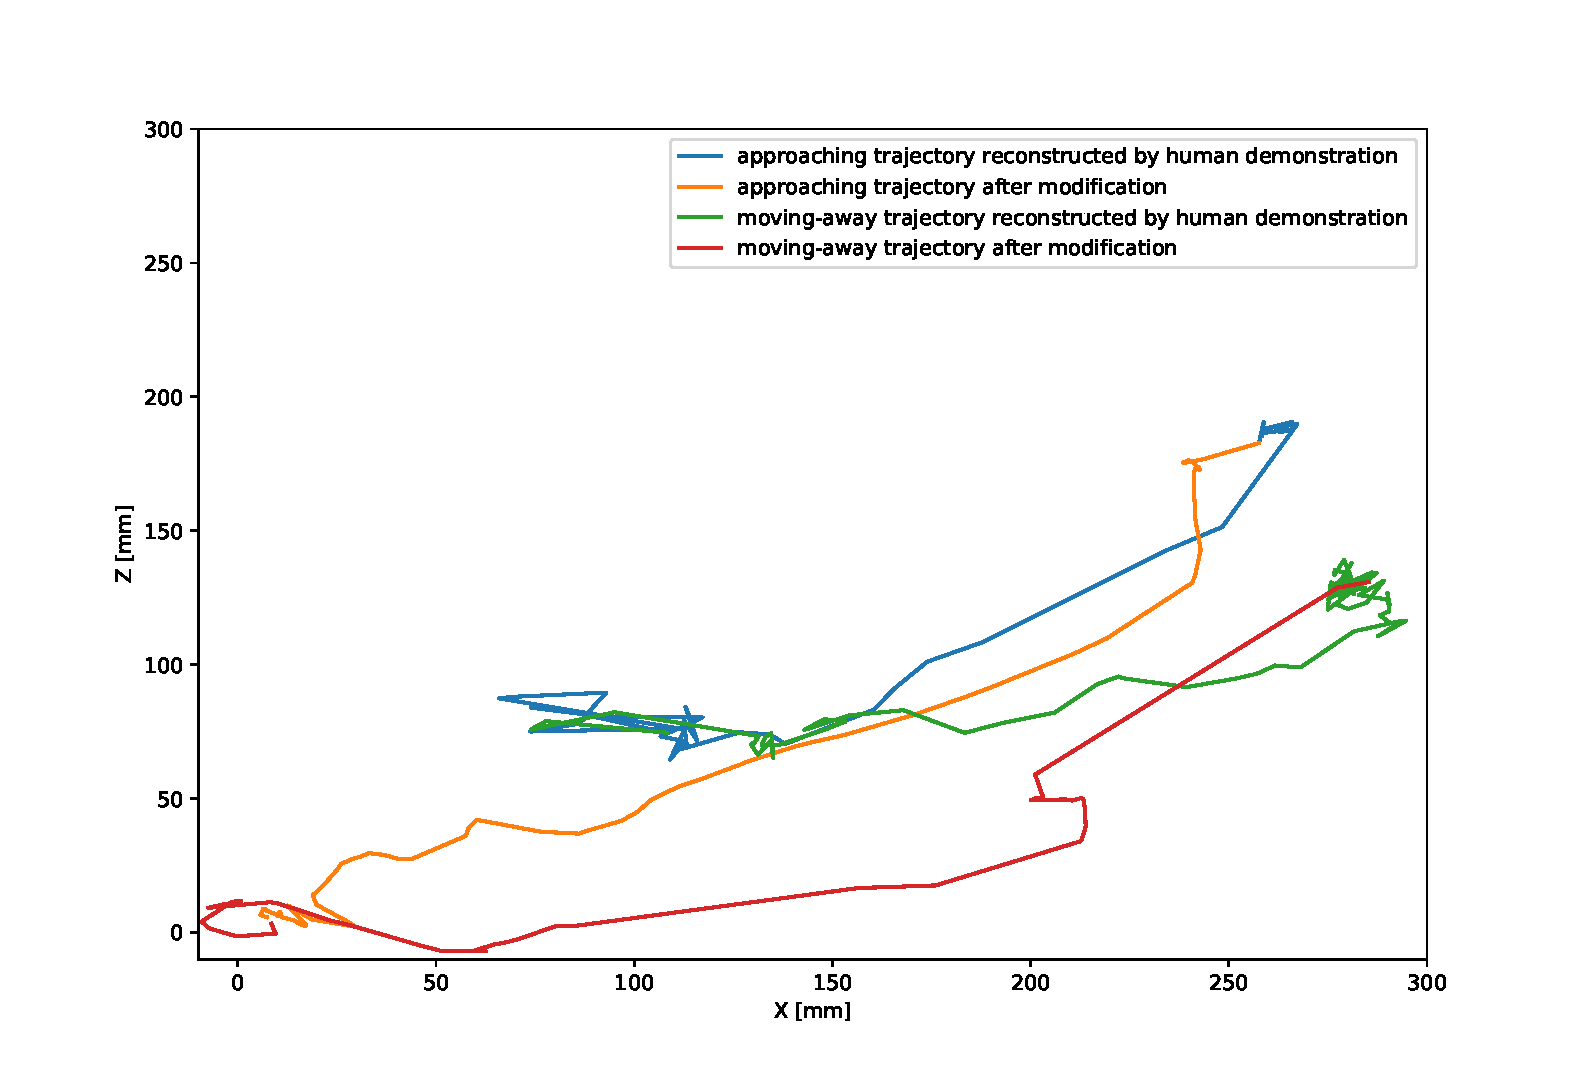
\includegraphics[width=0.80\columnwidth]{figs/trajectories}
%%   \caption{\small{A trajectory acquired by the demonstration and a trajectory acquired after the modification about ``push the stove button'' motion.}}
%%   \label{figure:target_pass}
%%  \end{center}
%%  \vspace{-5mm}
%% \end{figure}

\vspace{-3mm}
\begin{figure}[htbp]
 \begin{center}
  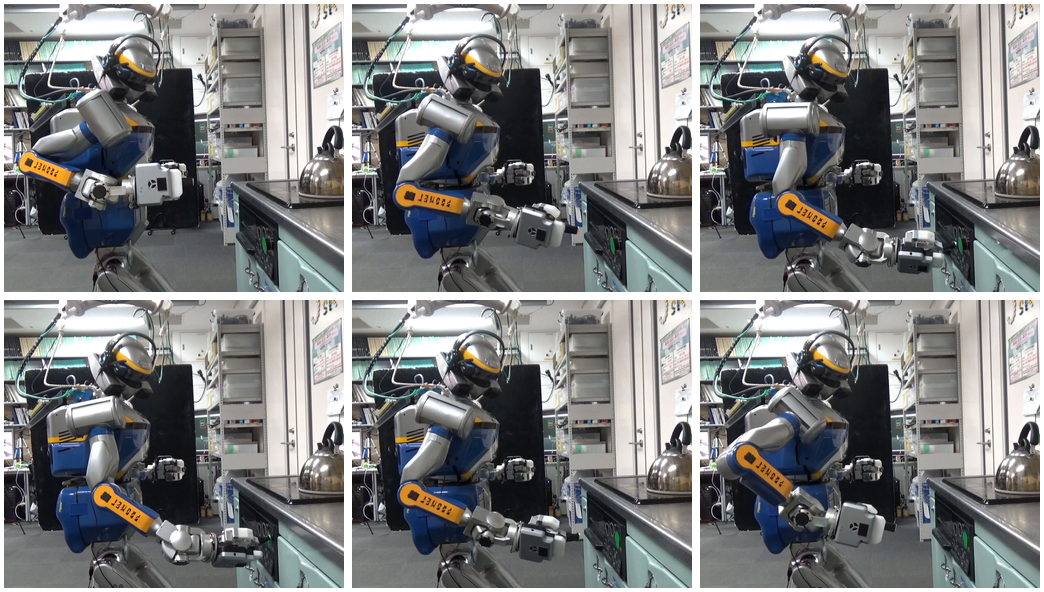
\includegraphics[width=0.80\columnwidth]{figs/push_button}
  \caption{\small{The snapshots during ``push the stove button'' motion by HRP-2}}
  \label{figure:experiment}
 \end{center}
 \vspace{-5mm}
\end{figure}
